\documentclass[11pt]{article}
\usepackage[a4paper,margin=2.2cm]{geometry}
\usepackage{amsmath,amssymb}
\usepackage{graphicx}
\usepackage{subcaption}
\usepackage{booktabs}
\usepackage{multirow}
\usepackage{xcolor}
\usepackage[colorlinks=true,linkcolor=blue]{hyperref}
\graphicspath{{clip_w1_assets/}}
\newcommand{\code}[1]{\texttt{#1}}

\title{\textbf{Honest-Side Gradient Clipping: Fixed Cap vs.\ Self-Calibrated}\\[2pt]
\large Fixed $C{=}21$ vs.\ ``clip to the first gradient'' (w1), all aggregators}
\author{ByzFL\_SNN}
\date{\today}

\begin{document}
\maketitle

\begin{abstract}
We compare two honest-side raw-gradient clipping mechanisms for Byzantine-robust FL on
\code{cnn\_mnist}: (i) a \emph{fixed} absolute cap $C=21$ (offline-derived from the honest
gradient ceiling), and (ii) a \emph{self-calibrated} cap where each client freezes its own
threshold from the L2 norm of its very first gradient (\code{w1}). Both are evaluated on the
identical grid across all four robust aggregators (best-over-aggregators, worst-over-attacks,
5 seeds). The headline result: \code{w1} clips far more aggressively (its cap
$\approx 3$--$5$, i.e.\ the pre-transient gradient norm, vs.\ the fixed $21$) and this
\emph{helps} at moderate heterogeneity ($\gamma{=}0.33$: $+0.15$ accuracy at $f{=}3$) but
\emph{hurts} at the extreme wall ($\gamma{=}0$, $f{=}5$). We also place both against the
calibrated fixed-cap family ($C\in\{7.7,17.6,21,26.7\}$ and per-layer).
\end{abstract}

\section{Setup}
\code{cnn\_mnist} (2 conv + 2 FC, ReLU), MNIST, DSGD, lr $0.15$, momentum $0.9$, wd $10^{-4}$,
batch $128$, $500$ steps, \textbf{5 seeds}. $n{=}10$ honest clients, $f\in\{0,\dots,5\}$
Byzantine. Heterogeneity $\gamma\in\{1.0,0.66,0.33,0.0\}$. Pre-aggregation NNM$\to$ARC;
aggregators \{GeometricMedian, CenteredClipping, TrMean, MultiKrum\}. Attacks \{Opt-ALIE,
SignFlipping, Opt-IPM\}. Every heatmap cell is \code{best\_test} $=$ worst case over attacks,
best over aggregators.

\section{The two mechanisms}
Both clip the \emph{raw} gradient (right after \code{backward()}, before the momentum
accumulator), via $g \mapsto g\cdot\min(1, C/\lVert g\rVert_2)$. They differ only in $C$.

\paragraph{Fixed cap (\code{gradclip21}).}
A single global constant $C=21$, identical for every client and every step, derived offline
as the honest gradient-norm ceiling (max over the no-attack baseline; reached at $\gamma{=}0$).

\paragraph{Self-calibrated warmup, \code{w1}.}
Each honest client observes only its first gradient, then freezes
\[
    C_{\text{self}} = \lVert g_1 \rVert_2 \cdot m \qquad (m=1.0,\ \text{frozen at step }1),
\]
and clips every later gradient to it. No probe, no SNN, no global constant. \textbf{Key point:}
the raw honest norm \emph{ramps up} from $\lVert g_1\rVert \approx 3$--$5$ to a transient peak
of $\sim$21--27 around step 40--55 before decaying. So \code{w1} freezes its cap \emph{below}
the transient peak, and therefore clips the entire honest transient down to $\sim$3--5 --- it
is a deliberately \emph{aggressive} absolute clip, roughly $4$--$7\times$ tighter than the
fixed $21$.

\section{Headline: fixed $C{=}21$ vs.\ w1}
\begin{figure}[h]
  \centering
  \begin{subfigure}{0.48\textwidth}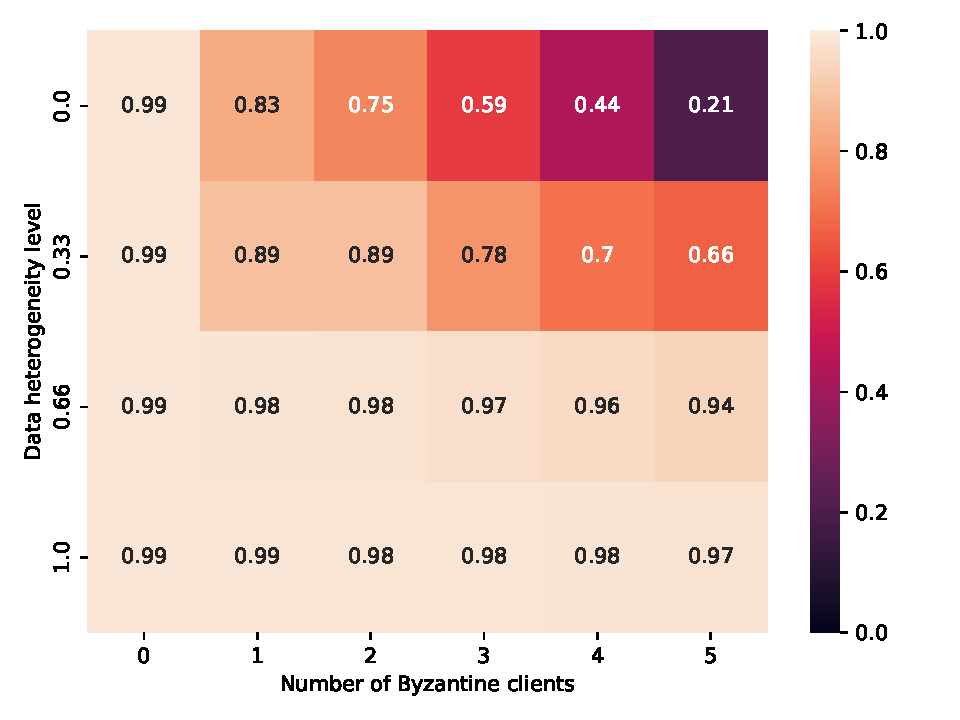
\includegraphics[width=\linewidth]{fixed21_best.pdf}
    \caption{Fixed cap $C=21$}\end{subfigure}\hfill
  \begin{subfigure}{0.48\textwidth}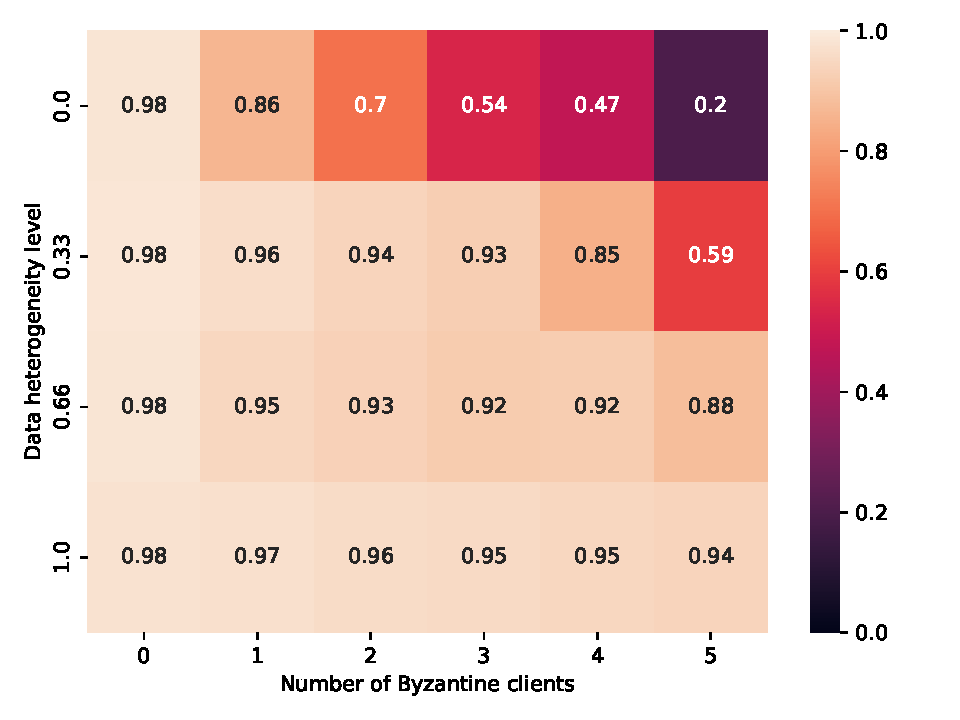
\includegraphics[width=\linewidth]{w1_best.pdf}
    \caption{Self-calibrated \code{w1} (clip to first gradient)}\end{subfigure}
  \caption{\code{best\_test} (worst-case over attacks, best over aggregators).}
\end{figure}

\begin{center}\small
\setlength{\tabcolsep}{5pt}
\begin{tabular}{@{}ll cccccc@{}}
\toprule
& & \multicolumn{6}{c}{$f=0,1,2,3,4,5$}\\ \cmidrule(l){3-8}
$\gamma$ & mech & 0 & 1 & 2 & 3 & 4 & 5\\
\midrule
\multirow{2}{*}{$0.0$}  & fixed 21 & 0.99 & 0.83 & \textbf{0.75} & 0.59 & 0.44 & \textbf{0.21}\\
                        & w1       & 0.98 & \textbf{0.86} & 0.70 & 0.54 & \textbf{0.47} & 0.20\\
\midrule
\multirow{2}{*}{$0.33$} & fixed 21 & 0.99 & 0.89 & 0.89 & 0.78 & 0.70 & \textbf{0.66}\\
                        & w1       & 0.98 & \textbf{0.96} & \textbf{0.94} & \textbf{0.93} & \textbf{0.85} & 0.59\\
\midrule
\multirow{2}{*}{$0.66$} & fixed 21 & 0.99 & \textbf{0.98} & \textbf{0.98} & \textbf{0.97} & \textbf{0.96} & \textbf{0.94}\\
                        & w1       & 0.98 & 0.95 & 0.93 & 0.92 & 0.92 & 0.88\\
\midrule
\multirow{2}{*}{$1.0$}  & fixed 21 & 0.99 & \textbf{0.99} & \textbf{0.98} & \textbf{0.98} & \textbf{0.98} & \textbf{0.97}\\
                        & w1       & 0.98 & 0.97 & 0.96 & 0.95 & 0.95 & 0.94\\
\bottomrule
\end{tabular}
\end{center}

\noindent\textbf{Reading it.} \code{w1} is markedly better at \emph{moderate} heterogeneity
($\gamma{=}0.33$: $+0.05$ to $+0.15$ across $f{=}1$--$4$, e.g.\ $0.93$ vs $0.78$ at $f{=}3$),
and slightly better at the hardest wall for low $f$ ($\gamma{=}0$, $f{=}1$/$f{=}4$). The
fixed cap wins at the very tip of the wall ($\gamma{=}0$, $f{=}5$: $0.66$ vs $0.59$ at
$\gamma{=}0.33$) and in the easy, low-heterogeneity regimes ($\gamma\in\{0.66,1.0\}$), where
aggressive clipping needlessly throttles honest progress ($-0.02$ to $-0.06$).

\section{Per-aggregator breakdown}
\begin{figure}[h]
  \centering
  \begin{subfigure}{0.24\textwidth}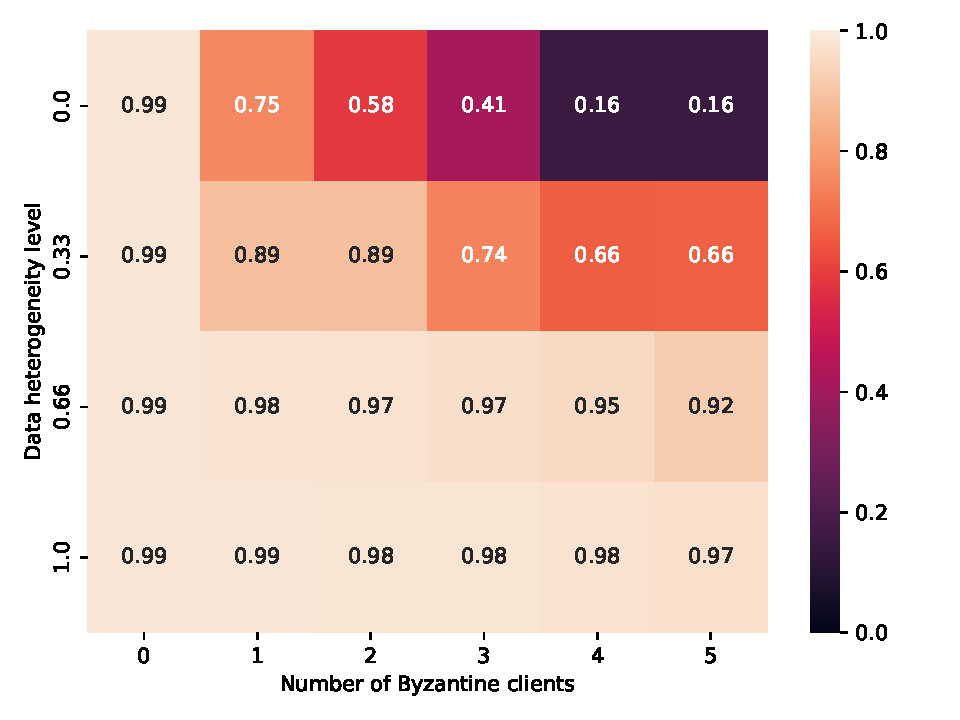
\includegraphics[width=\linewidth]{fixed21_GeometricMedian.pdf}\caption{GM}\end{subfigure}\hfill
  \begin{subfigure}{0.24\textwidth}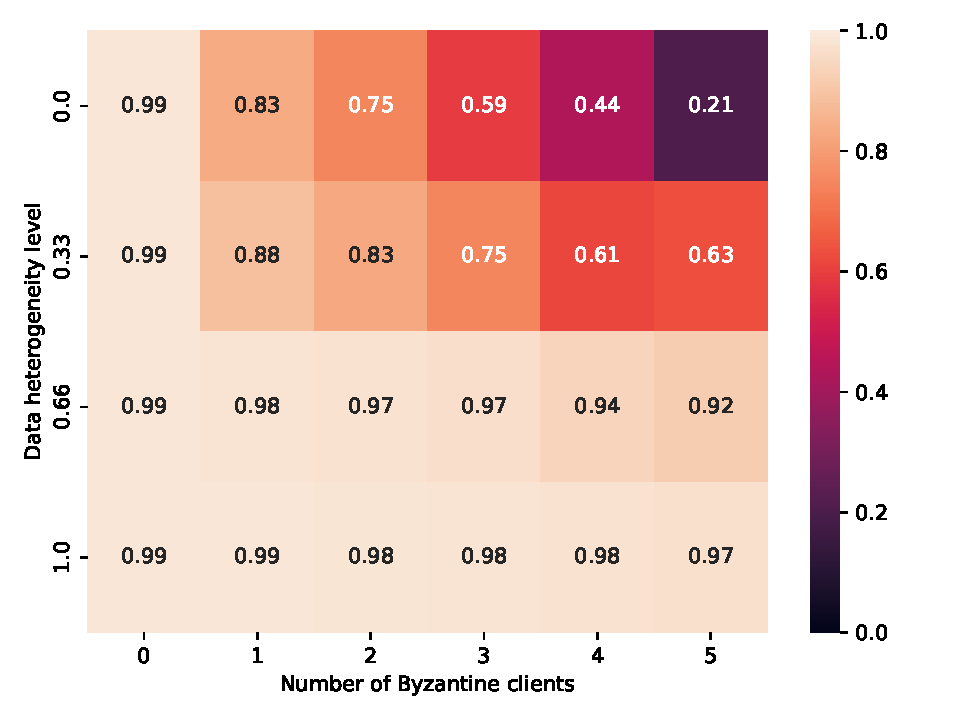
\includegraphics[width=\linewidth]{fixed21_CenteredClipping.pdf}\caption{CC}\end{subfigure}\hfill
  \begin{subfigure}{0.24\textwidth}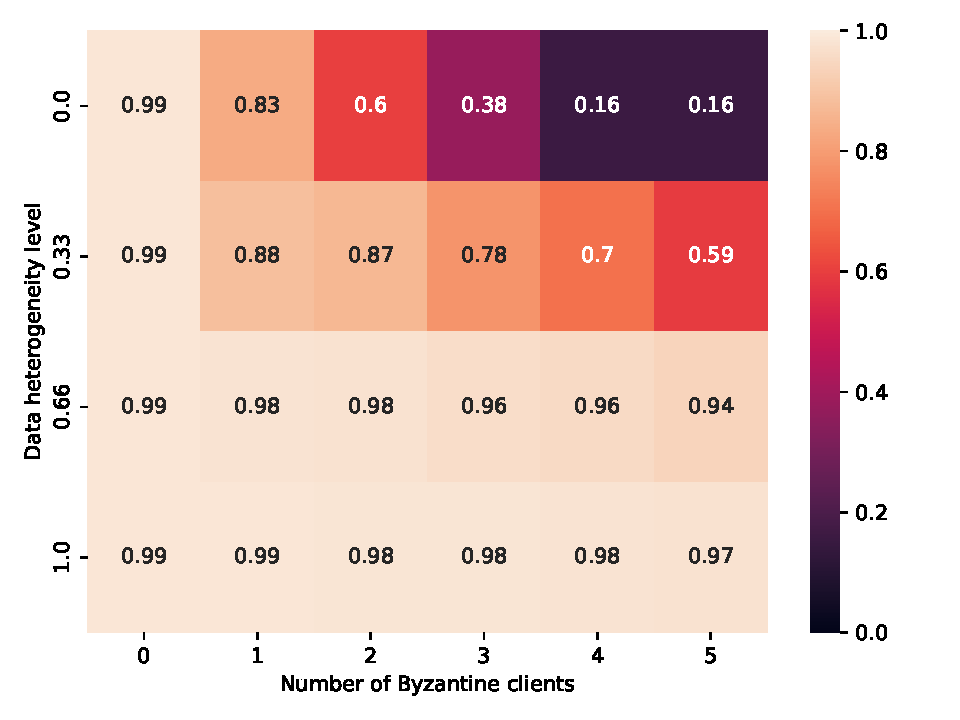
\includegraphics[width=\linewidth]{fixed21_TrMean.pdf}\caption{TrMean}\end{subfigure}\hfill
  \begin{subfigure}{0.24\textwidth}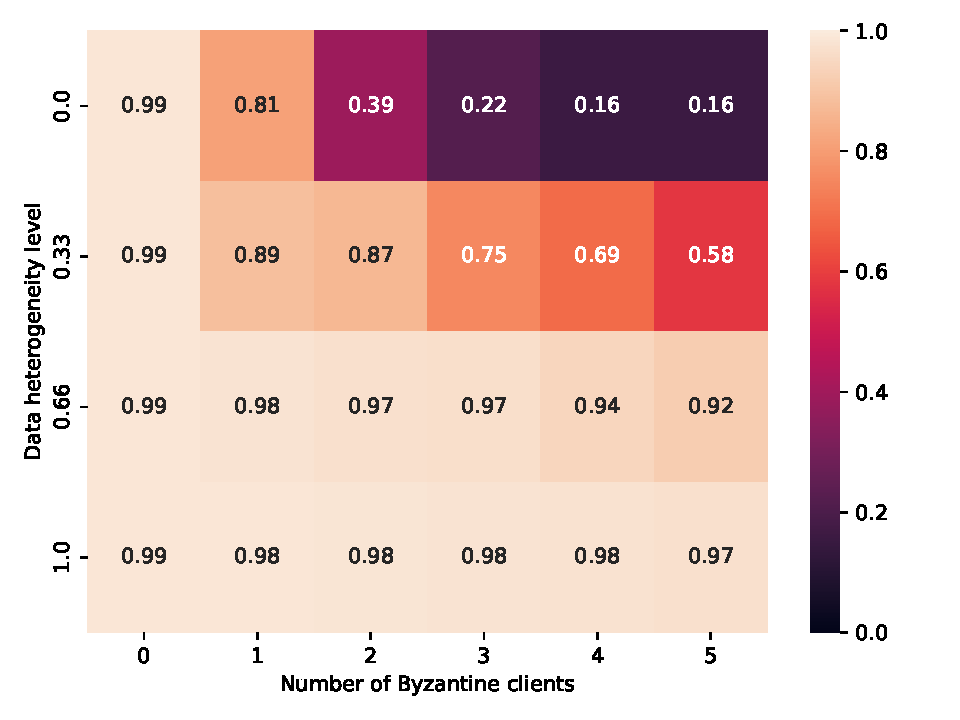
\includegraphics[width=\linewidth]{fixed21_MultiKrum.pdf}\caption{MultiKrum}\end{subfigure}
  \caption{Fixed $C=21$, per aggregator (worst-case over attacks).}
\end{figure}
\begin{figure}[h]
  \centering
  \begin{subfigure}{0.24\textwidth}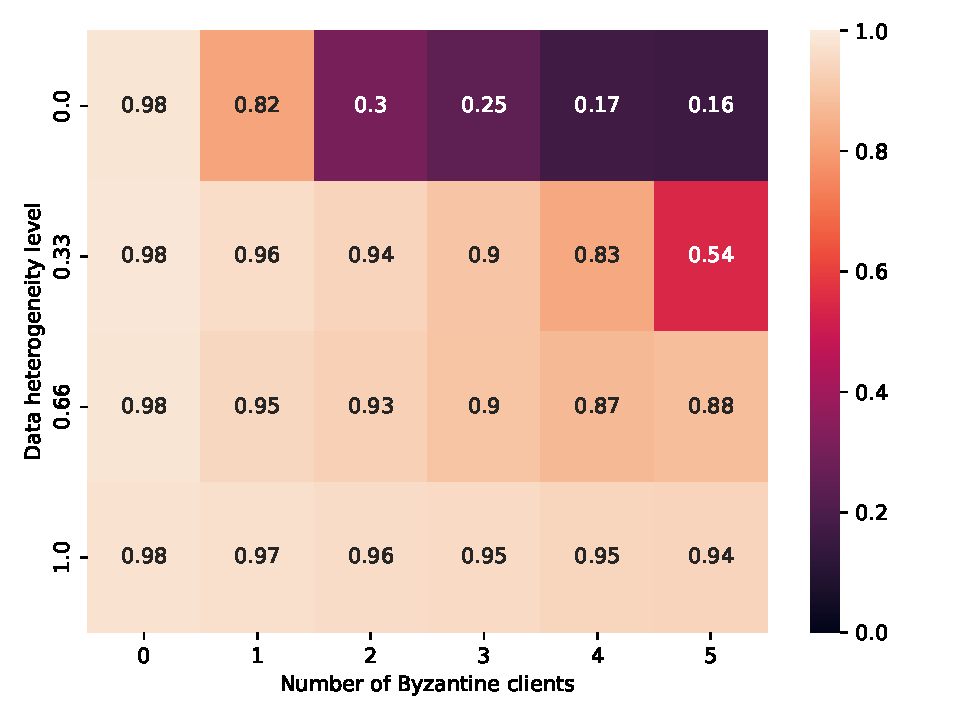
\includegraphics[width=\linewidth]{w1_GeometricMedian.pdf}\caption{GM}\end{subfigure}\hfill
  \begin{subfigure}{0.24\textwidth}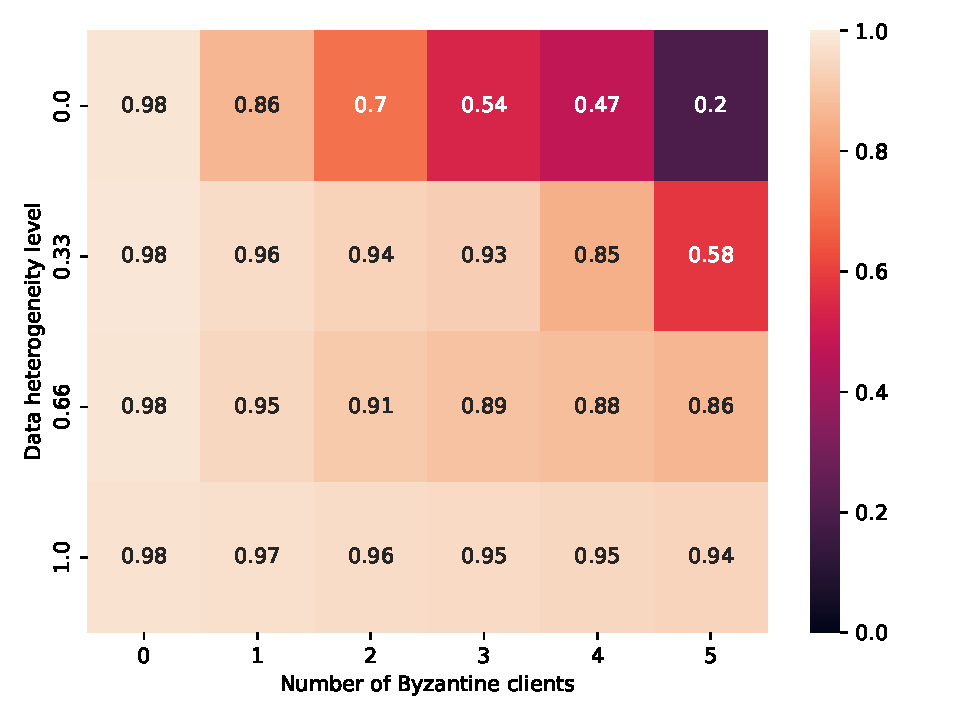
\includegraphics[width=\linewidth]{w1_CenteredClipping.pdf}\caption{CC}\end{subfigure}\hfill
  \begin{subfigure}{0.24\textwidth}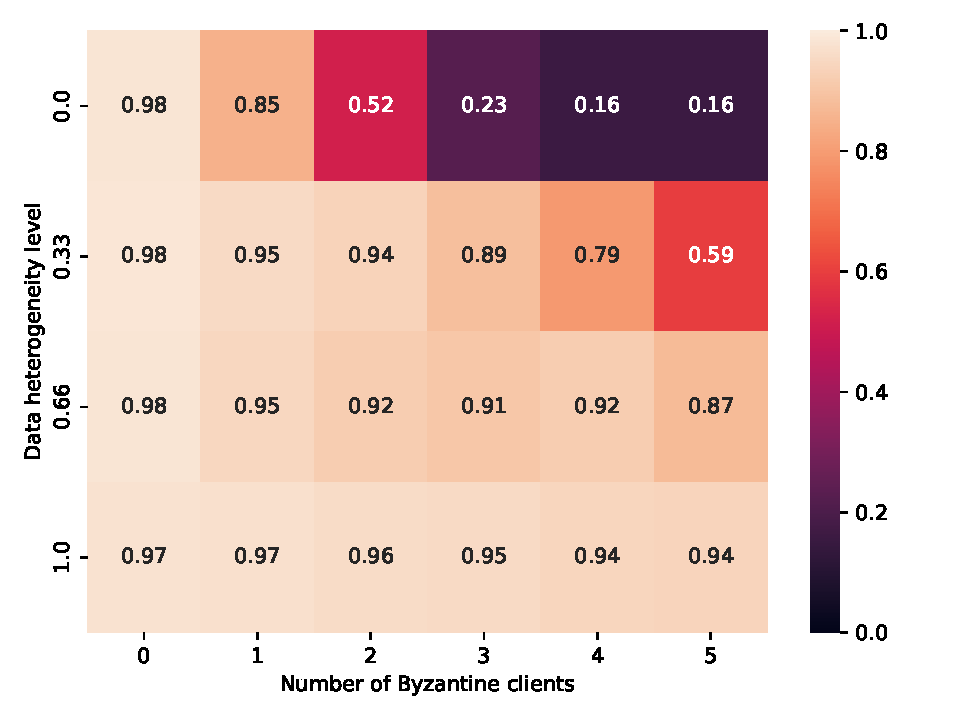
\includegraphics[width=\linewidth]{w1_TrMean.pdf}\caption{TrMean}\end{subfigure}\hfill
  \begin{subfigure}{0.24\textwidth}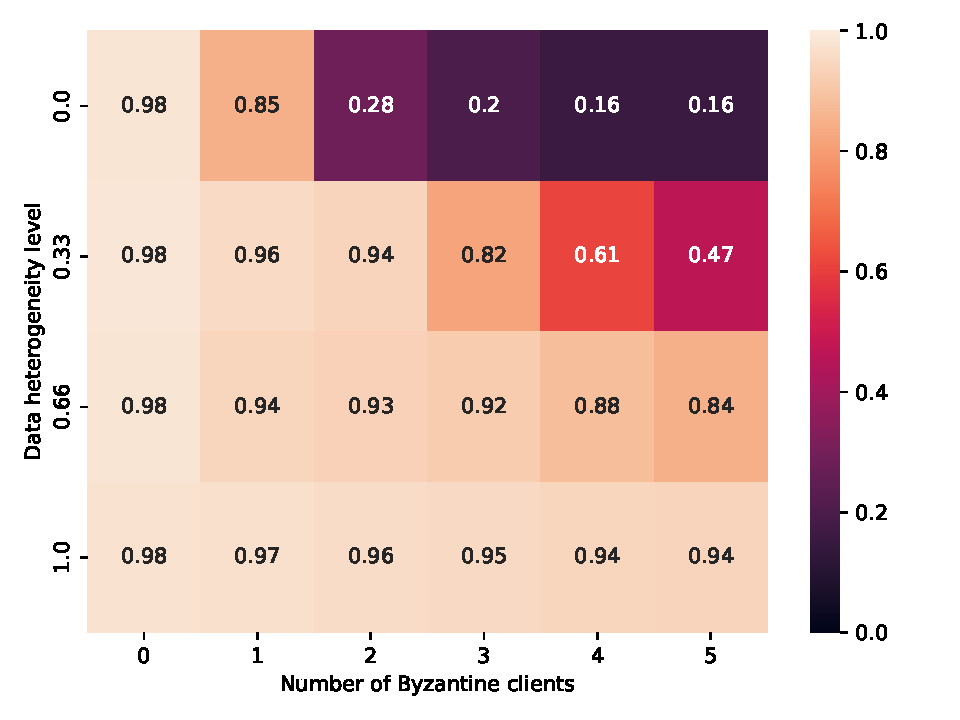
\includegraphics[width=\linewidth]{w1_MultiKrum.pdf}\caption{MultiKrum}\end{subfigure}
  \caption{Self-calibrated \code{w1}, per aggregator (worst-case over attacks).}
\end{figure}

\section{Against the calibrated fixed-cap family}
The fixed cap swept by value ($C\in\{7.7,17.6,21,26.7\}$, all algorithm-derived) plus the
per-layer variant, shown as \code{best\_test}. Tighter fixed caps trend toward \code{w1}'s
aggressive behaviour; \code{layerclip}'s $f{=}5$ column is a known crash (uniform $0$).
\begin{figure}[h]
  \centering
  \begin{subfigure}{0.32\textwidth}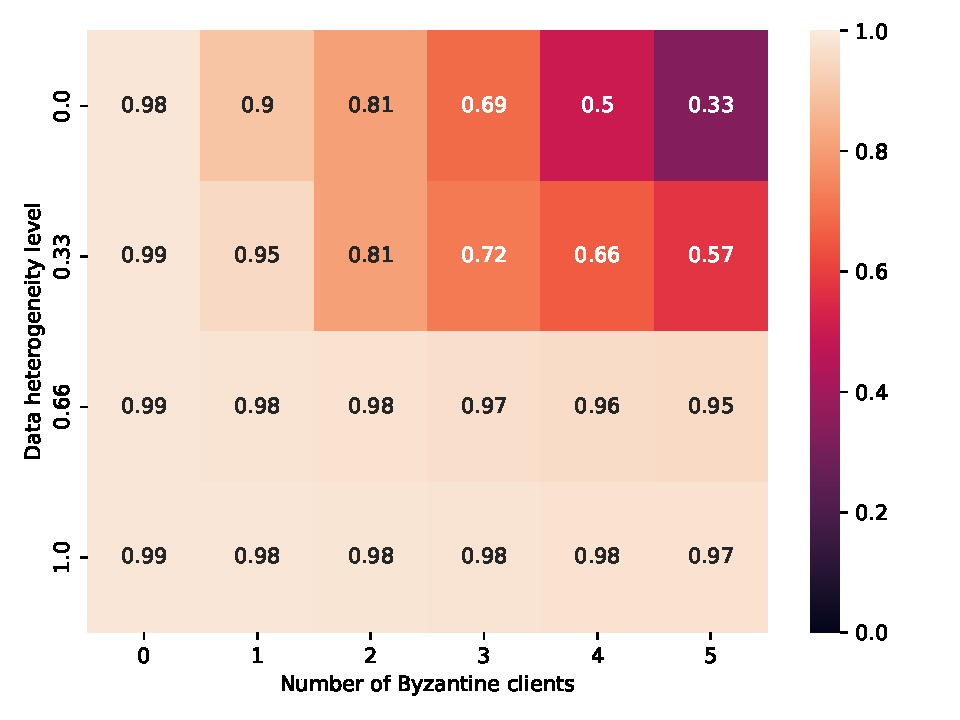
\includegraphics[width=\linewidth]{qlow_best.pdf}\caption{$C{=}7.7$ (qlow)}\end{subfigure}\hfill
  \begin{subfigure}{0.32\textwidth}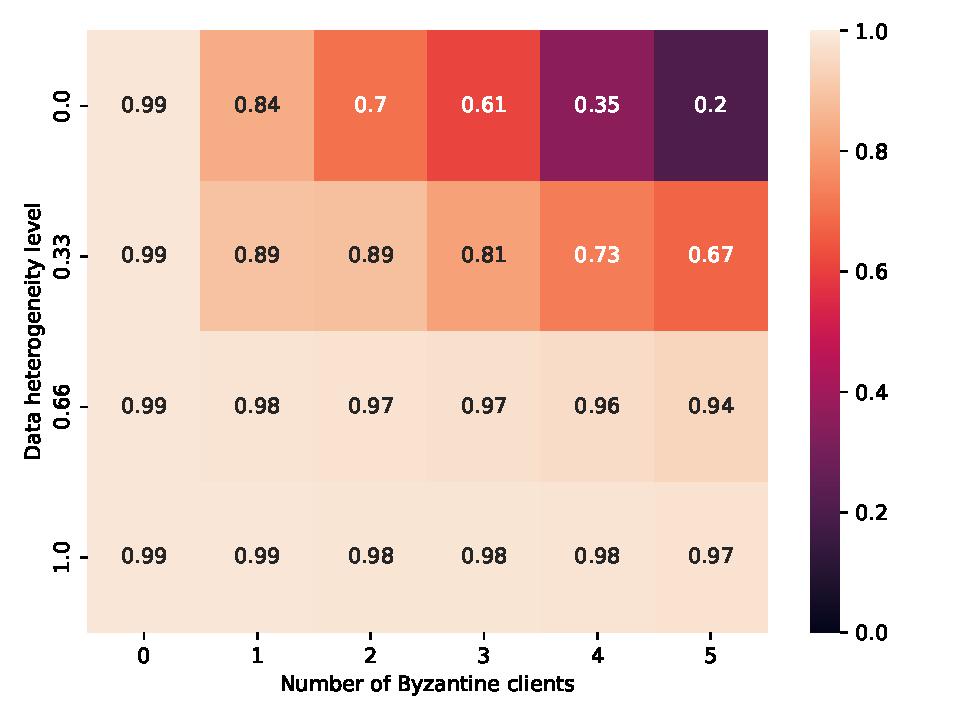
\includegraphics[width=\linewidth]{calib_best.pdf}\caption{$C{=}17.6$ (calib)}\end{subfigure}\hfill
  \begin{subfigure}{0.32\textwidth}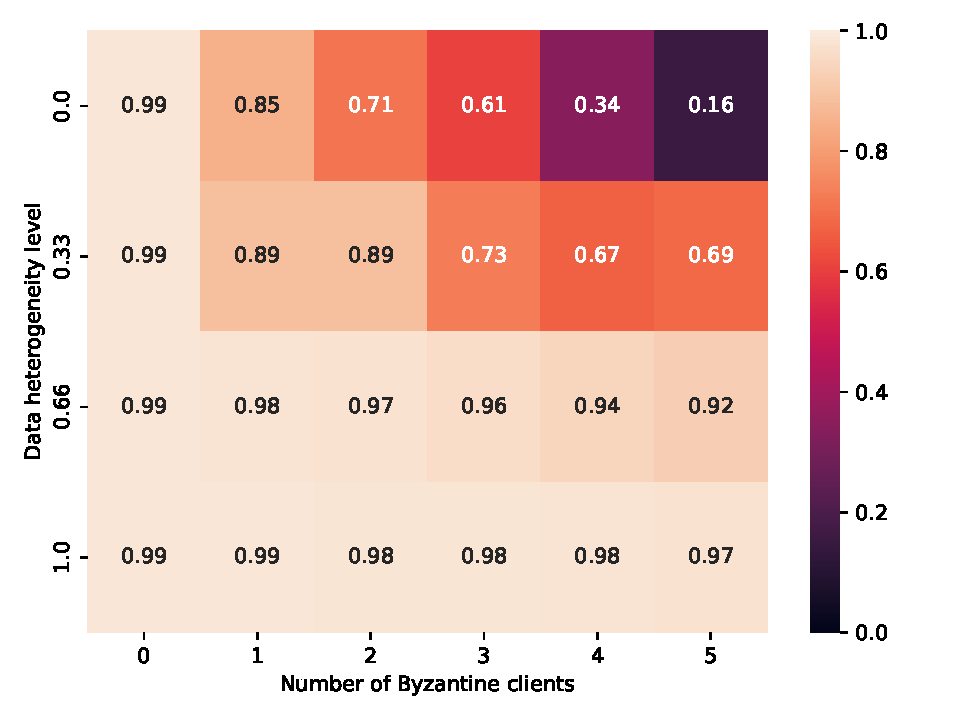
\includegraphics[width=\linewidth]{qhigh_best.pdf}\caption{$C{=}26.7$ (qhigh)}\end{subfigure}
  \\[4pt]
  \begin{subfigure}{0.32\textwidth}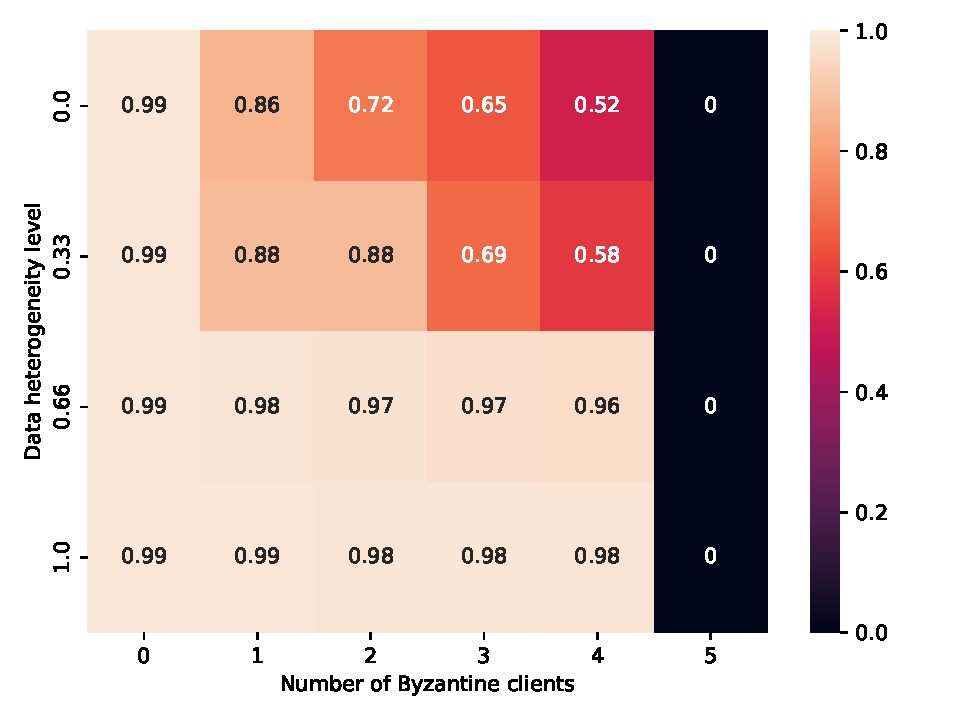
\includegraphics[width=\linewidth]{layerclip_best.pdf}\caption{per-layer}\end{subfigure}\hfill
  \begin{subfigure}{0.32\textwidth}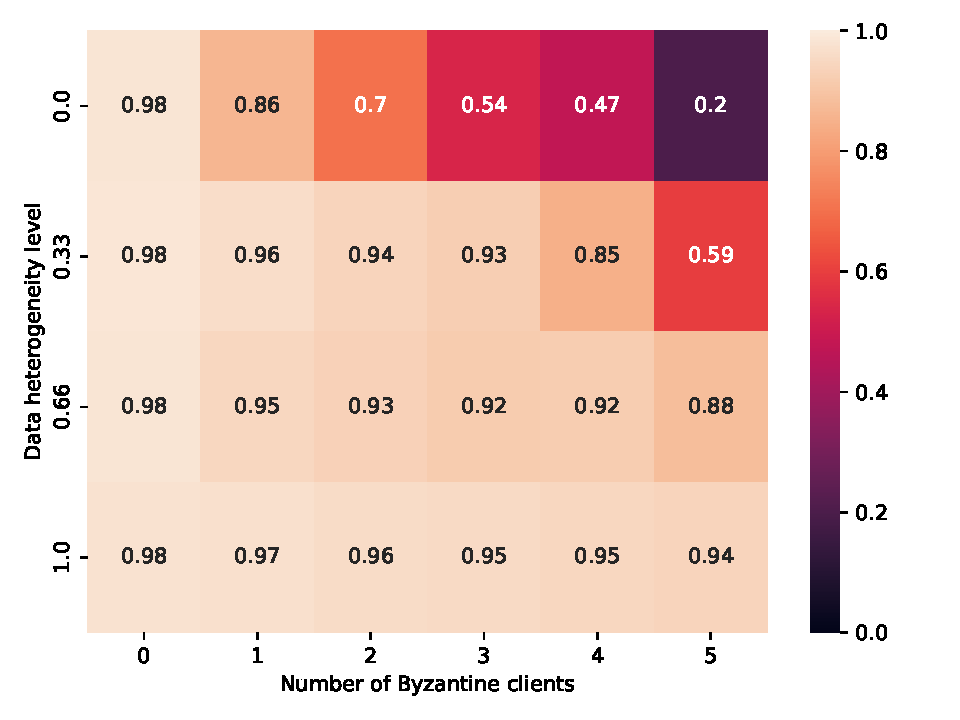
\includegraphics[width=\linewidth]{w1_best.pdf}\caption{\code{w1} (self-calibrated)}\end{subfigure}\hfill
  \begin{subfigure}{0.32\textwidth}\ \end{subfigure}
  \caption{Fixed-cap value sweep + per-layer + self-calibrated, all \code{best\_test}.}
\end{figure}

\section{Findings}
\begin{enumerate}\itemsep3pt
  \item \textbf{Aggressive clipping is a real lever at moderate heterogeneity.} \code{w1}
    (effective cap $\approx$ first-gradient norm $\approx 3$--$5$) beats the honest-ceiling
    fixed cap $21$ across $\gamma{=}0.33$, up to $+0.15$ accuracy. The dominant effect is
    \emph{how hard} you clip, not calibration to the honest ceiling.
  \item \textbf{But there is a heterogeneity-dependent optimum.} At the $\gamma{=}0$ tip and
    in the easy regimes, over-aggressive clipping costs accuracy: the fixed $21$ wins there.
    No single clip is best everywhere --- the cap$\leftrightarrow$robustness curve moves with
    $\gamma$.
  \item \textbf{Self-calibration reaches this for free.} \code{w1} needs no offline probe, no
    SNN, no global constant --- each client derives its cap online from its own first gradient
    --- yet it matches or beats the offline fixed cap in the regime that matters most
    (moderate non-iid). Caveat: the first-gradient cap is set while attacks are already
    present ($f$ fixed from step 1), a possible ``cap-poisoning'' surface not exercised by
    ALIE/SF/IPM but worth noting.
  \item \textbf{Shared wall.} Both collapse at $\gamma{=}0$, $f\ge2$ ($\approx0.2$--$0.7$):
    honest-side clipping tightens but does not remove the extreme-heterogeneity breakdown.
\end{enumerate}

\end{document}
